\documentclass[10pt,a4paper]{article}
\usepackage{amsmath,amssymb,amsthm,graphicx}
\usepackage{amsmath,amsthm,amssymb,mathtools,graphicx,xcolor,textcomp,multirow}
\usepackage[no-math]{fontspec}
\usepackage[linesnumbered,ruled,procnumbered]{algorithm2e}
\usepackage[colorlinks=true,hypertexnames=false]{hyperref}
\usepackage[capitalize]{cleveref}
\newtheorem{theorem}{Theorem}
\newtheorem{lemma}[theorem]{Lemma}
\newtheorem{definition}[theorem]{Definition}
\newtheorem{notation}[theorem]{Notation}
\newtheorem{proposition}[theorem]{Proposition}
\newtheorem{corollary}[theorem]{Corollary}
\newtheorem{conjecture}[theorem]{Conjecture}
\newtheorem{assumption}[theorem]{Assumption}
\newtheorem{fact}[theorem]{Fact}
\newtheorem{remark}[theorem]{Remark}
\newtheorem{claim}[theorem]{Claim}
\newtheorem{example}[theorem]{Example}
\newtheorem{problem}[theorem]{Problem}
\newtheorem{hypothesis}[theorem]{Hypothesis}
\newtheorem{observation}[theorem]{Observation}
\newcommand{\wh}{\widehat}
\newcommand{\wt}{\widetilde}
\newcommand{\ov}{\overline}
\newcommand{\eps}{\epsilon}
\newcommand{\N}{\mathbb{N}}
\newcommand{\A}{\mathcal{A}}

\newcommand{\Hil}{\mathcal{H}}
\newcommand{\F}{\mathbb{F}}
\newcommand{\R}{\mathbb{R}}
\renewcommand{\P}{\mathbb{P}}
\newcommand{\RHS}{\mathrm{RHS}}
\newcommand{\LHS}{\mathrm{LHS}}
\renewcommand{\d}{\mathrm{d}}
\renewcommand{\i}{\mathbf{i}}
\renewcommand{\varepsilon}{\lambda}
\renewcommand{\tilde}{\wt}
\renewcommand{\hat}{\wh}
\renewcommand{\eps}{\epsilon}
\newcommand{\sig}{\mathrm{sig}}
\newcommand{\high}{\mathrm{high}}
\newcommand{\bad}{\mathrm{bad}}
\newcommand{\diag}{\textrm{diag}}
\renewcommand{\d}{\mathrm{d}}
\newcommand{\ip}[2]{\langle {#1} , {#2} \rangle}
\newcommand{\norm}[1]{\| #1 \|}
\DeclareMathOperator*{\E}{{\mathbb{E}}}
\DeclareMathOperator*{\Var}{{\bf {Var}}}
\DeclareMathOperator*{\Sup}{{\bf {Sup}}}
\DeclareMathOperator*{\Z}{\mathbb{Z}}
%
\DeclareMathOperator*{\C}{\mathbb{C}}
\DeclareMathOperator{\supp}{supp}
\newcommand{\epsf}{\eta}
\newcommand{\ket}[1]{\left| #1 \right\rangle}
\newcommand{\bra}[1]{\left\langle #1 \right|}

\DeclareMathOperator{\poly}{poly}
\DeclareMathOperator{\polylog}{polylog}
\DeclareMathOperator{\nnz}{nnz}
\DeclareMathOperator{\rank}{rank}
\DeclareMathOperator{\new}{new}
\DeclareMathOperator{\pre}{pre}
\DeclareMathOperator{\old}{old}
\DeclareMathOperator{\tr}{tr}
\DeclareMathOperator*{\argmin}{arg\,min}
\newcommand{\ceil}[1]{\lceil #1 \rceil}
\newcommand{\floor}[1]{\lfloor #1 \rfloor}

\renewcommand{\S}{\mathcal{S}}
\newcommand{\U}{\mathcal{U}}
\newcommand{\id}{\mathrm{id}}



%
\newcommand{\ora}{\mathcal{O}}
\newcommand{\FG}{\mathrm{FG}}
\newcommand{\QFG}{\mathrm{QFG}}
\newcommand{\CP}{\ensuremath{\mathsf{CP}}}
\newcommand{\OV}{\ensuremath{\mathsf{OV}}}
\newcommand{\OVH}{\ensuremath{\mathsf{OVH}}}
\newcommand{\SAT}{\ensuremath{\mathsf{SAT}}}
\newcommand{\BCP}{\ensuremath{\mathsf{BCP}}}
\newcommand{\xiBCP}{(1+\xi)\text{-}\mathsf{BCP}}
\newcommand{\xiCP}{(1+\xi)\text{-}\mathsf{CP}}
\newcommand{\eCP}{\mathsf{CP}_{\epsilon}}
\newcommand{\eBCP}{\mathsf{BCP}_{\epsilon}}
\newcommand{\xieBCP}{(1+\xi)\text{-}\mathsf{BCP}_{\epsilon}}
\newcommand{\ZOV}{\ensuremath{\Z\text{-}\mathsf{OV}}}
\newcommand{\CRR}{\mathsf{CRR}}
\newcommand{\MA}{\mathsf{MA}}

\crefname{claim}{Claim}{Claims}
\crefname{procedure}{Procedure}{Procedures}


%
\SetAlgoProcName{Procedure}{Procedure}


\newcommand{\zo}{\{0,1\}}
\SetAlgoProcName{Procedure}{Procedure}
\allowdisplaybreaks
\AtBeginDocument{\author{\parbox{.95\textwidth}{\centering Scott Aaronson, Nai-Hui Chia, Han-Hsuan Lin,\\ Chunhao Wang, Ruizhe Zhang}}}
\title{Constant-dimensional quantum closest pair via history-independent data structures and quantum walks}
\author{Scott Aaronson, Nai-Hui Chia, Han-Hsuan Lin, Chunhao Wang, Ruizhe Zhang}
\date{doi:10.4230/LIPIcs.CCC.2020.16; CC BY 3.0 Unported}
\begin{document}
\maketitle
\noindent\textit{Editorial scope.} One algorithmic mechanism for constant-dimensional CP,with complete history-independent structures/quantum-walk proof and both single-shot/multiple-trial implementations. Dimension/precision variants and ED optimality are supporting consequences,not extra tasks.\par\medskip
\noindent\textit{Allowed standard prerequisites (editorial).}\begin{itemize}
\item Quantum query/QRAM model,Grover/minimum finding,MNRS quantum walk and element-distinctness lower bound. Formal Section2 definitions and Lemma22 framework retained. Cited standard quantum-walk/skip-list/permutation/error-amplification components remain background;all local data-structure algorithms,history-independence,error and complexity proofs retained. Full52 formal bibliography entries retained.
\end{itemize}\medskip
\setcounter{section}{1}
\setcounter{theorem}{5}
\section{Preliminaries}
\begin{definition}[Distance measure]
For any two vectors $a,b\in\R^d$, the distance between them in the $\ell_2$-metric is denoted by $\|a-b\|=\left(\sum_{i=1}^d|a_i-b_i|^2\right)^{1/2}$.
Their distance in the $\ell_0$-metric (Hamming distance) is denoted by 
$\|a-b\|_0=|\{i\in[d]:a_i\neq b_i\}|$, i.e.,
the number of coordinates on which $a$ and $b$ differ.
\end{definition}


\subsection{Quantum query model}

We consider the quantum query model in this work. Let $X:=\{x_1,\dots,x_n\}$ be a set of $n$ input points and $\ora_X$ be the corresponding oracle. We can access the $i$-th data point $x_i$ by making the query 
\begin{align}
    \ket{i}\ket{0} \xrightarrow{\ora_X} \ket{i}\ket{x_i},  
\end{align}
and we can make queries to elements in $X$ in superposition. Note that $\ora_X$ is an unitary transformation in the formula above. Hence, a quantum algorithm with access to $\ora_X$ can be represented as a sequence of unitary transformations. 

Consider a quantum algorithm $\A$ with access to an oracle $\ora$ and a initial state $\ket{0}:= \ket{0}_{Q}\ket{0}_{A}\ket{0}_W$, where the registers $Q$ and $A$ are for the queries and the answers from the oracle, and the register $W$ is the working space which is always hold by $\A$.  Then, we can represent the algorithm as 
\begin{align}
    U_T \ora U_{T-1}\cdots\ora U_1  \ket{0}. 
\end{align}
Let $\ket{\psi}_i= U_i\ora \cdots \ora U_1\ket{0}:= \sum_{i,z} \ket{i}_Q\ket{0}_A\ket{z}_W$ be the state right before applying the $i$-th $\ora$, then
\begin{align}
    \ora \ket{\psi}_i:= \sum_{i,z} \ket{i}_Q\ket{x_i}_A\ket{z}_W.
\end{align}
\subsection{Quantum subroutine for unstructured searching and minimum finding}

\begin{definition}[Unstructured search]
Given a set $P$ of $n$ elements in $\{0,1\}$, decide whether there exists a $1$ in $P$. 
\end{definition}

\begin{theorem}[Grover's search algorithm~\cite{r24,r37}]\label{thm:grover_algo}
There is a quantum algorithm for unstructured search with running time $O(\sqrt{n})$.
\end{theorem}

By \cref{thm:grover_algo} and BBBV's argument \cite{r9}, the quantum time complexity of unstructured search is $\Theta(\sqrt{n})$. We can also get a $\tilde{O}(\sqrt{n})$ quantum algorithm for minimum finding by combining Grover's search algorithm and binary search.
\begin{theorem}[Quantum minimum finding~\cite{r23}]\label{thm:mim}
There is a quantum algorithm that finds from a set of $n$ elements with values in $\mathbb{R}$, the index of the minimum element of the set, with success probability $\frac{1}{2}$ and run time $\tilde{O}(\sqrt{n})$.
\end{theorem}

\subsection{Problem definitions}
In this subsection, we first formally define  $\OV$, $\CP$, and $\BCP$. Then we show the folklore algorithms for $\CP$, $\BCP$, and $\OV$ by Grover's algorithm, which run in time $\tilde{O}(n)$. 
\begin{definition}[Orthogonal Vectors, $\OV$]\label{def:OV}
Given two sets $A,B$ of $n$ vectors in $\mathbb \{0,1\}^d$ as input, find a pair of vectors $a\in A$, $b\in B$ such that
$\ip{a}{b}=0$, where the inner product is taken in $\mathbb{Z}$.\footnote{Our definition is slightly different than some of the literature, for example, \cite{r18}, which is searching among pairs inside one set. Those two definitions are equivalent up to constant in complexities.}
\end{definition}

We denote $\OV$ with input length $n$ and dimension $d$ as $\OV_{n,d}$. We will use this notation when we need to specify the parameters in the following sections.  

\begin{definition}[Closest Pair Problem, $\CP$]
Given a set $P$ of $n$ points in $\mathbb R^d$ and a distance measure $\Delta$, find a pair of distinct points $a,b\in P$ such that $\Delta(a,b)$ is the smallest among all distinct pairs in $P$.
\end{definition}
Similar to $\OV$, we denote $\CP$ with input length $n$ and dimension $d$ as $\CP_{n,d}$. We will use this notation when the parameters in the following sections are required to be specified. Note that in this work, we consider $\Delta(a, b) = \norm{a-b}$ as the distance measure for \textsf{CP} and \textsf{BCP}.

\begin{definition}[Bichromatic Closest Pair Problem, \textsf{BCP}]
Given two sets $A,B$ of $n$ points in $\mathbb R^d$ and a distance measure $\Delta$, find a pair of points $a\in A$, $b\in B$ such that 
\begin{align}
    \Delta(a,b)= \min_{a\in A,b\in B} \Delta(a,b).
\end{align}
\end{definition}
We also define an approximate version of $\BCP$ as follows.
\begin{definition}[$(1+\xi$)-approximate Bichromatic Closest Pair Problem, $\xiBCP$]
Given two sets $A,B$ of $n$ points $\in \mathbb R^d$ and a distance measure $\Delta$, find a pair of points $a\in A$, $b\in B$ such that 
\begin{align}
    \Delta(a,b) \leq (1+\xi)\min_{a\in A,b\in B} \Delta(a,b).
\end{align}
\end{definition}
Same as $\CP$, we use $\BCP_{n,d}$ and $\xiBCP_{n, d}$ to specify the parameters. 

\begin{definition}[Element Distinctness Problem, \textsf{ED}]
  Let $f:[n] \rightarrow [m]$ be a given function. Decide whether there exist distinct $i, j\in[n]$ such that $f(i) = f(j)$.
\end{definition}

For this problem, Ambainis \cite{r5} gave a quantum algorithm with time complexity $\tilde{O}(n^{2/3})$, which matches the lower bound proved by Aaronson and Shi \cite{r1} up to a polylogarithmic factor.

\begin{theorem}\label{cor:trivial_alg}
There are $\tilde{O}(n)$-time quantum algorithms for $\CP$ and $\BCP$ when $d=O(\poly\log n)$.
\end{theorem}
\begin{proof}
We can solve $\CP$ and $\BCP$ by searching the minimum distance through all pairs by the algorithm of \cref{thm:mim}. There are $O(n^2)$ pairs and checking each pair took $O(d)$ time, so the total running time is $O(nd)$. For $d=O(\poly\log n)$, the time complexity equals to $\tilde{O}(n)$.
\end{proof}

\subsection{Fine-grained complexity}

As we have mentioned earlier in the introduction, a fine-grained reduction from problem $\mathsf{P}$ to $\mathsf{Q}$ with conjectured lower bounds $p(n)$ and $q(n)$, respectively, has the property that if we can improve the $q(n)$ time for $\mathsf{Q}$, then we can also improve the $p(n)$ time for $\mathsf{P}$. We give the formal definition by Williams~\cite{r46} in below. 

\begin{definition}[Fine-grained reduction, \cite{r46}]\label{def:fg}
Let $p(n)$ and $q(n)$ be non-decreasing functions of $n$. Problem $\mathsf{P}$ is ($p,q$)-reducible to problem $\mathsf{Q}$, denoted as $(\mathsf{P},p)\leq_{\FG} (\mathsf{Q},q)$, if for every $\epsilon$, there exist $\delta>0$, an algorithm $R$ for solving $\mathsf{P}$ with access to an oracle for $\mathsf{Q}$, a constant $d$, and an integer $k(n)$, such that for every $n\ge 1$, the algorithm $R$ takes any instance of $\mathsf{P}$ of size $n$ and 
\begin{itemize}
    \item $R$ runs in at most $d\cdot (p(n))^{1-\delta}$-time, 
    \item $R$ produces at most $k(n)$ instances of $\mathsf{Q}$ adaptively, that is, the $j$th instance $X_j$ is a function of $\{(X_i,y_i)\}_{1\leq i<j}$ where $X_i$ is the $i$th instance produced and $y_i$ is the answer of the oracle for $\mathsf{Q}$ on instance $X_i$, and 
    \item the sizes $n_i$ of the instances $X_i$ for any choice of oracle answers $y_i$ obeys the inequality
    \begin{align}\label{eq:fgr}
        \sum_{i=1}^{k(n)} (q(n_i))^{1-\epsilon} \leq d\cdot (p(n))^{1-\delta}.
    \end{align}
\end{itemize}
\end{definition}

Let $(\mathsf{P},p)\leq_{\FG} (\mathsf{Q},q)$ for some non-decreasing function $p(n)$ and $q(n)$. If for every $\eps > 0$, we can solve problem $\mathsf{Q}$ in time $q(n)^{1-\epsilon}$ with probability $1$ for all input length $n$, then there exists a $\delta>0$ such that we can solve the problem $\mathsf{P}$ in time $p(n)^{1-\delta}$ 
by \cref{eq:fgr}.

Here are some known results about fine-grained reductions.
\begin{theorem}[\cite{r29,r49}]\label{thm:classical_fg}
\begin{align}
    (\mathsf{CNF\text{-}SAT}_{n},2^n)\leq_{\FG} (\OV_{n_1,d_1},n_1^2)\leq_{\FG} (\BCP_{n_2,d_2},n_2^2)\leq_{\FG} (\CP_{n_3,d_3},n_3^2),
\end{align}
where $d_1=\Theta(\log n_1)$, $d_2=\Theta(\log n_2)$ and $d_3=(\log  n_3)^{\Omega(1)}$.
\end{theorem}

\begin{remark}
The second reduction from $\OV$ to $\BCP$ has been improved to $d_2 = 2^{O(\log^* n)}$ by Chen~\cite{r17}.
\end{remark}

There are several plausible hypotheses in fine-grained complexity, which can imply conditional hardness results for many interesting problems. We first give the definition of the strong exponential time hypothesis (SETH). 
\begin{hypothesis}[Strong Exponential Time Hypothesis, \textsf{SETH}]
For every $\epsilon > 0$, there exists a $k = k(\epsilon) \in \N$ such that no algorithm can solve $k$-$\SAT$ (i.e., satisfiability on a CNF of width $k$) in $O(2^{(1 - \epsilon)m})$ time where $m$ is the number of variables. Moreover, this holds even when the number of clauses is at most $c(\epsilon) \cdot m$ where $c(\epsilon)$ denotes a constant that depends only on $\epsilon$.
\end{hypothesis}

Another popular conjecture is the orthogonal vector hypothesis (\textsf{OVH}):
\begin{definition}[Orthogonal Vector Hypothesis, \textsf{OVH}]
For every $\epsilon > 0$,  
there exists a $c\ge 1$ such that $\OV_{n,d}$ requires $n^{2-\epsilon}$ time when $d=c\log n$.
\end{definition}

\begin{remark}
Under SETH, we can have the following conclusions from \cref{thm:classical_fg}: 
\begin{itemize}
    \item $\OVH$ is true. 
    \item For all $\epsilon>0$, there exists a $c>0$ such that $\BCP_{n,c\log n}$ cannot be solved by any randomized algorithm in time $O(n^{2-\epsilon})$.
    \item For all $\epsilon>0$, there exists a $c>0$ such that $\CP_{n,(\log n)^c}$ cannot be solved by any randomized algorithm in time $O(n^{2-\epsilon})$.
\end{itemize}
\end{remark}

\subsection{The framework for quantum walk search}
\label{sec:qw-framework}
In this subsection, we review the quantum walk framework for the Markov chain search problem and demonstrate how to use it to solve the element distinctness problem. For simplicity, we use the transition matrix $P$ to refer to a Markov chain, where $P = (p_{xy})_{x, y \in X}$ for $X$ being the state space of $P$ and $p_{xy}$ being the transition probability from $x$ to $y$. An irreducible and ergodic Markov chain has a unique stationary distribution $\pi$, which is also the unique eigenvector of $P$ with eigenvalue 1. Let $M \subseteq X$ be a set of marked elements. In the Markov chain search problem, the objective is to find an $x \in M$. We can perform the following actions: setup, sampling from the $\pi$ with cost $\mathsf{S}$; update, making a transition with cost $\mathsf{U}$, and checking whether the current state is marked or not with cost $\mathsf{C}$. To solve the search problem classically, we perform a random walk as follows. Start from a point sampled from $\pi$ and check if it is marked. If not, make a number of transitions on $P$ until it mixes, and then check again. We then repeat this process until a marked state is found. The cost of this random walk algorithm is $O(\mathsf{S} + \frac{1}{\varepsilon}(\frac{1}{\delta}\mathsf{U} + \mathsf{C}))$, where $\varepsilon:= |M|/|X|$ and $\delta$ is the spectral gap of $P$.

Quantum analogues of random walks, namely, quantum walks, have been developed for solving different problems. In 2003, Ambainis~\cite{r5} proposed a quantum walk algorithm for solving the element distinctness problem. His algorithm also solves the Markov chain search problem on the Johnson graph with cost $O(\mathsf{S} + \frac{1}{\sqrt{\varepsilon}}(\frac{1}{\sqrt{\delta}}\mathsf{U} + \mathsf{C}))$. In 2004, Szegedy~\cite{r45} gave a quantum walk algorithm for more generalized Markov chains with cost $O(\mathsf{S} + \frac{1}{\sqrt{\varepsilon\delta}}(\mathsf{U} + \mathsf{C}))$. We can view Szegedy's quantum walk as a quantum counterpart of a random walk, where one checks the state after each transition. Szegedy's quantum walk only detects the presence of a marked state, but cannot find one without extra costs. In 2006, Magniez et al.~\cite{r33} proposed a quantum walk search framework that unified the advantages of the quantum walks in~\cite{r5} and~\cite{r45}. In this quantum walk framework, we can perform the following operations:
\begin{itemize}
  \item \textbf{Setup:} with cost $\mathsf{S}$. preparing the initial state $\ket{\pi} = \frac{1}{\sqrt{|X|}}\sum_{x}\sqrt{\pi_x}\ket{x}$.
  \item \textbf{Update:}  with cost $\mathsf{U}$. applying the transformation $\ket{x}\ket{0} \mapsto \ket{x}\sum_{y\in X}\sqrt{p_{xy}}\ket{y}$.
  \item \textbf{Checking:} with cost $\mathsf{C}$, applying the transformation: $\ket{x} \mapsto \big\{\begin{smallmatrix} -\ket{x} \quad &\text{if $x\in M$} \\ \ket{x} \quad &\text{otherwise.}\end{smallmatrix}$
\end{itemize}
The main result of \cite{r33} is summarized as follows.
\begin{lemma}[\cite{r33}]
  \label{lem:framework}
  Let $P$ be an irreducible and ergodic Markov chain $P$ on $X$. Let $M \subseteq X$ be a subset of marked elements. Let $\varepsilon: = |M|/|X|$ and $\delta$ be the spectral gap of $P$. Then, there exists a quantum algorithm that with high probability, determines $M$ is empty or finds an $x \in M$ with cost $O(\mathsf{S} + \frac{1}{\sqrt{\varepsilon}}(\frac{1}{\sqrt{\delta}}\mathsf{U} + \mathsf{C}))$.
\end{lemma}

To solve the element distinctness problem, we define a Markov chain, following the work~\cite{r5,r11,r28}. The state space $X$ is all subsets of $[n]$ with size $r$. The Markov chain is based on the Johnson graph on $X$, where an edge is connecting $S$ and $S'$ if and only if $|S \cap S'| = r-1$. The transition probability on each edge is hence $\frac{1}{r(n-r)}$. A state $S$ is marked when there exist distinct $i, j \in S$ such the $i^{th}$ and the $j^{th}$ items are the same. The Markov chain has spectral gap $\delta \geq 1/r$ (see~\cite{r28}) and it is easy to verify that $\varepsilon \geq \binom{n-2}{r-2}/\binom{n}{r} = O(r^2/n^2)$. If we only consider the query complexity, the setup procedure costs $r$ queries, the update procedure costs one query, and the checking procedure does not cost any query. Choosing $r = n^{2/3}$ yields the optimal query complexity $O(n^{2/3})$.



\setcounter{section}{3}
\setcounter{theorem}{39}
\setcounter{figure}{2}
\section{Closest pair in constant dimension}
\label{sec:cp}

In this section, we show that there exist almost-optimal quantum algorithms for $\CP$ in constant dimension. The main result is the following theorem, which is a direct consequence of \cref{cor:main_cp,thm:cp_constant}.
\begin{theorem}
For any constant dimension, the quantum time complexity for $\CP$ is $\tilde{\Theta}(n^{2/3})$. 
\end{theorem}


Our approach to solve \textsf{CP} is first  reducing to the decision version of the problem, and then apply quantum walk algorithms to solve the decision version. We define the decision version of \textsf{CP},  $\eCP$, as follows. 
\begin{definition}[$\eCP$]
Given a set of points $P\subset \mathbb{R}^{d}$ and $\epsilon\in \mathbb{R}$, find a pair $a,b\in P$ such that $\|a-b\|\leq \epsilon$ if there is one and returns \textsf{no} is no such pair exists. 
\end{definition}
The reduction from $\CP$ to $\eCP$ is given by the following lemma.
\begin{lemma}
  \label{lemma:cp-ecp}
Let $m$ be the number of bits needed to encode each coordinate as a bit string and $d$ be the dimension.
Given an oracle $\ora$ for $\eCP$, there exists an algorithm $A^{\ora}$  that runs in time and query complexity $O(m+\log d )$ that solves the $\CP$. 
\end{lemma}
\begin{proof}
Let $(P,\delta)$ be an instance of the $\CP$.  We first pick an arbitrary pair $a_0,b_0\in P$ and compute $\Delta(a_0,b_0)$. Then, we set $\epsilon$ to be $\Delta(a_0,b_0)/2$ and run the oracle $\ora$ to check whether there exists a distinct pair with distance less than $\Delta(a_0,b_0)/2$ or not. If there exists such a pair, which we denote as $(a_1,b_1)$, then we set $\epsilon=\Delta(a_1,b_1)$ and call $\ora$ to check again. If there is no such pair, then we set $\epsilon=3\Delta(a_0,b_0)/4$ and call $\ora$. We run this binary search for $m+\log d$ iterations. Finally, the algorithm outputs the closest pair.  
\end{proof}

In classical setting, point location is an important step in solving the closest-pair problem, especially the dynamic version. For the quantum algorithm, as walking on the Markov chain, we repeatedly delete a point and add a new point. Hence, in each step, the first thing is to determine the location of the new added point.    

For simplicity, we assume that $m=O(\log n)$, which is the number of digits of each coordinate of the points. By translation, we can further assume that all the points are lying in $[0,L]^d$, where $L=O(2^m) = \poly(n)$. 

Since we are considering $\eCP$, one simple way of point location is to discretize the whole space into a hypergrid, which is defined as follows: 

\begin{definition}\label{def:hypergrid}
Let $d, \epsilon, L>0$. A hypergrid $G_{d,\epsilon,L}$ in the space $[0,L]^d$ consists of all  $\eps$-boxes 
\begin{align}
    g := [a_1,b_1)\times [a_2,b_2)\times \cdots \times [a_d,b_d), 
\end{align}
such that
$b_1-a_1=\cdots =b_d-a_d=\epsilon/\sqrt{d}$ \footnote{The diagonal length of an $\eps$-box is $\epsilon$.}, and $a_i$ is divisible by $\epsilon$ for all $i\in [d]$. 
\end{definition}

For each point $p_i\in [0,L]^d$, we can identify the $\epsilon$-box that contains it using the function $\id(p_i):[0,L]^d\rightarrow \{0,1\}^{d\log (L/\epsilon)}$:
\begin{align}\label{eq:id_fcn}
    \id(p_i)=\big(\left\lfloor p_i(1)/w\right\rfloor, \left\lfloor p_i(2)/w\right\rfloor, \dots, \left\lfloor p_i(d)/w\right\rfloor\big),
\end{align}
where $w=\frac{\epsilon}{\sqrt{d}}$ is the width of the $\eps$-box. The number of bits to store $\id(p_i)$ is $d\cdot \log(L/w)=O(d\cdot \log(L))$.
Since all the points in an $\epsilon$-box have the same $\id$, we also use this $g(\id(p))$ to denote this $\epsilon$-box containing $p$.

For the ease of our analysis, we define the neighbors of a hypergrid.
\begin{definition}\label{defn:kneighbor}
  Let $\epsilon\in \mathbb{R}$. Let $g_1, g_2$ be two $\eps$-boxes in a hypergrid where $\id(g_1) = (x_1,\dots,x_d)$ and $\id(g_2) = (x'_1,\dots,x'_d)$. We say that $g_1$ and $g_2$ are each other's \emph{$\epsilon$-neighbor} if 
\begin{align}
    \sqrt{\sum_{i=1}^d \|x_i-x'_i\|^2} \leq \epsilon
\end{align}
\end{definition}

Note that the number of $\epsilon$-neighbors of a $\epsilon$-box is at most $(2\sqrt{d}+1)^d$. We also have the following observation:
\begin{observation}\label{obs:2step}
Let $p_1,p_2\in [0,L]^d$ be any two distinct points.  
\begin{itemize}
    \item If $p_1$ and $p_2$ are in the same $\epsilon$-box, then $\Delta(p_1, p_2) \leq \epsilon$.
    \item If $\Delta(p_1, p_2)\leq \epsilon$, then $g(\id(p_1))$ must be an $\epsilon$-neighbor of $g(\id(p_2))$. 
\end{itemize} 
\end{observation}

To solve $\eCP$ with quantum walk, we need data structures to keep track of the pairs that have distance at most $\epsilon$. The desired data structure should have size $\tilde{O}(n^{2/3})$, insertion/deletion time $O(\log n)$, and one should be able to check whether there exist pairs of distance at most $\epsilon$ in time $O(\log n)$. In addition, as pointed out in~\cite{r5}, the data structure should have the following two properties:
\begin{itemize}
  \item the data structure should have the bounded \emph{worst-case} performance rather than \emph{average-case} performance;
  \item the representation of the data structure should be history-independent, i.e., the data is uniquely represented regardless of the order of insertions and deletions.
\end{itemize}

We need the first property since the data structure may take too long for some operations, and this is not acceptable. The second property is required because, otherwise, the interference of quantum states would be messed up. In~\cite{r5}, a hash table and a skip list is used to for solving the element distinctness problem using quantum walks. In~\cite{r11}, a simpler data structure, namely, a radix tree, is used to achieve the same performance. More details of using a radix tree to solve the element distinctness can be found in~\cite{r28}. Similar to the quantum data structure model in~\cite{r5,r11,r28}, we need the \emph{quantum random access gate} to efficiently access data from a quantum memory, whose operation is defined as:
\begin{align}
    \label{eq:qram-gate}
    \ket{i, b, z_1,\dots, z_m} \mapsto \ket{i, z_i, z_1, \ldots, z_{i-1}, b, z_{i+1}, z_m},
\end{align}
where $\ket{z_1,\dots, z_m}$ is some data in a quantum memory with $m$ qubits. We assume this operation takes $O(\log m)$ time.


In the remainder of this section, we present two quantum algorithms for solving $\eCP$. The data structures of both versions are based on the \textit{augmented radix tree}, which we discuss in detail in the following subsection.

\subsection{Radix tree for at most one solution}
\label{sec:radixtree}
The purpose of the augmented radix tree is to quickly locate the points in an $\epsilon$-box given its id. An ordinary radix tree is a binary tree that organizes a set of keys which are represented as binary strings. Each edge is labeled by a substring of a key and each leaf is labeled by a key such that concatenating all the labels on the path from the root to a leaf yields the key for this leaf. In addition, for each internal node, the labels of the two edges connecting to two children start with different bit. Note that in this definition, we implicitly merge all internal nodes that have only one child. The radix tree is uniquely represented for any set of keys. An example of a radix tree is shown as \cref{fig:radix-tree}.

\begin{figure}[t]
  \centering
  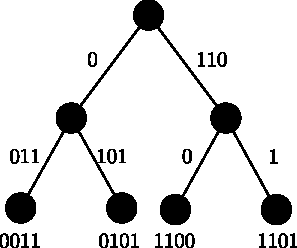
\includegraphics[width=0.3\textwidth]{radix-tree.pdf}
  \caption{The uniquely represented radix tree that stores the keys $\{0011, 0101, 1100, 1101\}$.} \label{fig:radix-tree}
\end{figure}

Our basic radix tree is essentially the one in~\cite{r11,r28} with modification on the nodes' internal structure. We highlight the extra information stored in the radix tree.
First we use a \emph{local counter} to store the number of points in this $\epsilon$-box; second, we use a \emph{flag} in each leaf node to indicate whether there is a point in this $\epsilon$-box that is in some pair with distance at most $\epsilon$. The flag bit in an internal node is the $\mathrm{OR}$ of the ones in its children. The local counter in each internal node is the sum of the local counters in its children. We also store at most two points that are in the $\epsilon$-box corresponding to this node. More precisely, let $S$ be a subset of indices of the input points. We use $\tau(S)$ to denote the radix tree associated with $S$.
Then, $\tau(S)$ consists of at most $r\ceil{\log r}$ nodes. Each node consists of the following registers:
\begin{align}
  \mathcal{D} \times \mathcal{M}_1 \times \mathcal{M}_2 \times \mathcal{M}_3 \times \mathcal{C} \times \mathcal{F} \times \mathcal{P}_1 \times \mathcal{P}_2,
\end{align}
where $\mathcal{D}$ stores the id of an $\epsilon$-box for a leaf (and a substring of an id for an internal node) using $O(d\log(L/\epsilon))$ bits. $\mathcal{M}_1, \mathcal{M}_2$, and $\mathcal{M}_3$ use $O(\log n)$ bits to store the pointers to its parent, left child, and right child, respectively as well as the labels of the three edges connecting them to this node, $O(\log n)$ bits to store the labels of the three edges incident to it. $\mathcal{C}$ uses $O(\log n)$ bits to store the local counter. $\mathcal{F}$ stores the flag bit. $\mathcal{P}_1$ and $\mathcal{P}_2$ stores the coordinates of at most two points in this $\epsilon$-box, which takes $O(d\log L)$ bits. The two points are stored in ascending order of their indices.

We need to pay attention to the layout of $\tau(S)$ in memory. We use three times more bits than needed to store $\tau(S)$, this will ensure that there are always more than $1/3$ of the bits that are free. We divide the memory into cells where each cell is large enough to store one leaf node of $\tau(S)$. Besides $\tau(S)$, we also store a bitmap $\mathcal{B}$, which takes $O(\log n)$ bits to encode the current free cells (with ``1'' indicating occupied and ``0'' indicating free). To make the radix tree history-independent, we use a quantum state which is the uniform superposition of basis states $\ket{\tau(S), B}$ for all possible valid layout of $\tau(S)$ and it corresponds to the bitmap $\mathcal{B}$.

Insertion and deletion from $\tau(S)$ takes $O(\log n)$ time. Checking the presence of an $\epsilon$-close pair takes constant time --- we just need to read the flag bit in the root. Preparing the uniform superposition of all $i \in S$ can be done in $O(\log n)$ time by performing a controlled-rotation on each level of the radix tree where the angles are determined by the local counters in the two children of a node.

In the following subsections, we present the two versions of our algorithms. The first version invokes the quantum walk framework only once and its data structure maintains the existence of an $\epsilon$-close pair. The second version uses a much simpler data structure, but it is only capable of handling $\eCP$ with a unique solution. Hence it requires invoking the quantum walk framework multiple times to solve the general $\eCP$. These two quantum algorithms have almost the same time complexity. 

\subsection{Single-shot quantum walk with complicated data structure}
\label{sec:one-shot}
To handle multiple solutions, our data structure is a composition of an augmented radix tree, a hash table, and a skip list. We give a high-level overview of our data structure as follows. Recall that by the discretization of the space into $\epsilon$-boxes,  it is possible that a pair of points in different $\epsilon$-boxes have distance at most $\epsilon$, but one only needs to check $(2\sqrt{d}+1)^d$ $\epsilon$-neighbors to detect such a case. We maintain a list of points for each nonempty $\epsilon$-box in an efficient way. A hash table is used to store the tuple $(i, p_i)$ which is used to quickly find the point $p_i$, given its index $i$. The points are also stored in a skip list for each nonempty $\epsilon$-box, ordered by its index $i$, which allows for quick insertion and deletion of points. Each $\epsilon$-box is encoded into a unique key, and a radix tree is used to store such key-value pairs, where the value is associated with a skip list. The flag bits in this radix tree maintain the presence of an $\epsilon$-close pair.

In the following, we present the details of the data structure and show it has all the desired properties.

\paragraph{Hash table.}
The hash table we use is almost the same as the one used in~\cite{r5}, except that we do not store the $\floor{\log r}$ counters in each bucket to facilitate the diffusion operator (which is handled easily here in the quantum walk on a Johnson graph). Our hash table has $r$ buckets, where each bucket contains $\ceil{\log n}$ entries. We use a fixed hash function $h(i) = \floor{ir/n}+1$ to hash $\{1, \ldots, n\}$ to $\{1, \ldots, r\}$. That is, for $j\in [r]$, the $j$-th bucket contains the entries for $(i, p_i)$ in ascending order of $i$, where $i \in S$ and $h(i) = j$. 

The entry for $(i, p_i)$ contains the tuple $(i, p_i)$ and $\ceil{\log n} + 1$ pointers to other entries. These pointers are used in the skip list which we will describe below. The memory size of each entry is hence $O(\log^2n + d\log L)$ and there are $O(r\log n)$ entries. Therefore, the hash table uses $O(rd\log^3(n + dL))$ qubits. 

It is possible that more than $\ceil{\log n}$ points are hashed into the same bucket. However, as shown in~\cite{r5}, this probability is small.

\paragraph{Skip list.}
The skip list we use closely follows that in~\cite{r5}, except that the elements $p_i$ in our skip list is ordered by its index $i$. We construct a skip list for each $\epsilon$-box containing at least one point to store the points in it. For each $i \in S$, $p_i$ belongs to exactly one skip list. 
Also, for $i \in S$, we randomly assign a level $\ell_i \in [0, \ldots, \ell_{\max}]$ where $\ell_{\max} = \ceil{\log n}$. The skip list associated with a $\epsilon$-box has $\ell_{\max}+1$ lists, where the level-$\ell$ list consists of all $i \in S$ such that $\ell_i \geq \ell$ and $p_i$ is in this $\epsilon$-box. Hence, the level-0 list consists of all $i \in S$ for $p_i$ in this $\epsilon$-box. Each element of the level-$\ell$ list has a specific pointer to the next element in this level, or to 0 if there is no next element. Each skip list contains a start entry that does not contain any $(i, p_i)$ information but $\ell_{\max}+1$ pointers to the first element of the each level. This start entry is stored in a leaf node of the augmented radix tree (which we will describe below) corresponding to this $\epsilon$-box. In each skip list, we do not allocate memory for each node. Instead, each pointer is pointing to an entry of the hash table. The pointers are stored in the hash table (for the internal entries of each level) and in the radix tree (for the start entry). An example of a skip list is shown in \cref{fig:skip-list}.

\begin{figure}[t]
  \centering
  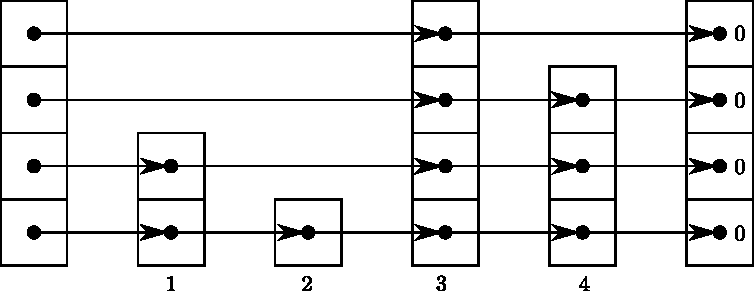
\includegraphics[width=0.6\textwidth]{skip-list.pdf}
  \caption{An example of a skip list that stores $\{1, 2, 3, 4\}$.} \label{fig:skip-list}
\end{figure}

Given $i\in S$, we can search for $p_i$ as follows. We start from the start entry of the level-$\ell_{\max}$ list and traverse each element until we find the last element $j_{\ell_{\max}}$ such that $j_{\ell_{\max}} < i$. Repeat this for levels $\ell_{\ell_{\max}-1}, \ldots, \ell_0$ and at each level start from the element that ended the previous level. At level-$0$, we obtain the element $j_0$. Then, the next element of $j_0$ is where $p_i$ should be located (if it is stored in this skip list) or be inserted.

Each $i \in S$ is randomly assigned a level $\ell_i$ at the beginning of computation that does not change during the computation. More specifically, $\ell_i = \ell$ with probability $1/2^{\ell+1}$ for $\ell < \ell_{\max}$ and with probability $1/2^{\ell_{\max}}$ for $\ell = \ell_{\max}$. This can be achieved using $\ell_{\max}$ hash functions $h_1, \ldots, h_{\ell_{\max}} : [n] \rightarrow \{0, 1\}$. In this way, each $i \in [n]$ has level $\ell<\ell_{\max}$ if $h_1(i) = \cdots = h_\ell(i) = 1$ but $h_{\ell+1}(i) = 0$; and it has level $\ell_{\max}$ if $h(i) = \cdots = h_{\ell_{\max}}(i) = 1$. In this quantum algorithm, we use an extra register to hold the state $\ket{h_1,\ldots,h_{\ell_{\max}}}$ which is initialized to a uniform superposition of all possible such functions from a $d$-wise independent family of hash functions (see~\cite[Theorem 1]{r5}) for $d = \ceil{4 \log n + 1}$. During the execution of the quantum algorithm, a hash function from the hashing family is chosen depending on the state in this register.

At first glance, the skip list has the same role as the hash table -- finding $p_i$ given index $i$. 
However, they have very different purposes in our algorithm. Recall that each nonempty $\epsilon$-box is associated with a skip list, which is used to quickly insert and delete a point in this $\epsilon$-box. The number of points in this $\epsilon$-box can be as small as one and as large as $r$ (in the extreme case where all the points are in the same $\epsilon$-box).
Hence, we cannot afford to have a fixed length data structure (such as a hash table or a sorted array) to store these points. In addition, to support quick insertion and deletion, a skip list is a reasonable choice (against an ordinary list). The purpose of the hash table can be viewed as a uniquely represented memory storing all the $r$ points that can be referred to by the skip lists.

\paragraph{Augmented radix tree.}
We augment the radix tree described in \cref{sec:radixtree} to handle multiple solution. In this augmented radix tree, we do not need the registers $\mathcal{P}_1$ and $\mathcal{P}_2$. Instead, we use $\ceil{\log n}$ pointers $\mathcal{L}_1, \ldots, \mathcal{L}_{\ceil{\log n}}$ as the start entry of a skip list. These pointers uses $O(\log^2 n)$ bits. In addition, we use an \emph{external counter} in the leaf nodes to record whether there is a point in other $\epsilon$-boxes that is at most $\epsilon$-away from a point in this $\epsilon$-box, which uses $O(\log n)$ bits. More formally, let $\tau'(S)$ be the augmented radix tree associated with $S$. 
Each node of $\tau'(S)$ consists of the following registers
\begin{align}
  \mathcal{D} \times \mathcal{M}_1 \times \mathcal{M}_2 \times \mathcal{M}_3 \times \mathcal{E} \times \mathcal{C} \times \mathcal{F} \times \mathcal{E} \times \mathcal{L}_1 \times \cdots \times \mathcal{L}_{\ceil{\log n}}.
\end{align}

Next, we present how to perform the required operations on $S$ with our data structure.

\paragraph{Checking for $\epsilon$-close pairs.}To check the existence of an $\epsilon$-close pair, we just read the flag in the root of the radix tree. If the flag is set, there is at most one $\epsilon$-close pair in $S$, and no such pairs otherwise. This operation takes $O(1)$ time.

\paragraph{Insertion.} 
Given $(i, p_i)$, we perform the insertion with the following steps:
\begin{enumerate}
  \item Insert this tuple into the hash table.
  \item Compute the id, $\id(p_i)$, of the $\epsilon$-box which $p_i$ belongs to. Denote this $\epsilon$-box by $g(\id(p_i))$.
  \item Using $\id(p_i)$ as the key, check if this key is already in $\tau'(S)$, if so, insert $i$ into the skip list corresponding to $g(\id(p_i))$; otherwise, first create a uniform superposition of the addresses of all free cells into another register, then create a new tree node in the cell determined by this address register and insert it into the tree. The pointers for the start entry of the skip list is initially set to 0. Insert $i$ into this skip list. Let $\tau'(S, g(\id(p_i))$ denote the leaf node in $\tau'(S)$ corresponding to $g(\id(p_i))$.
  \item Increase the local counter $\mathcal{C}$ in $\tau'(S, g(\id(p_i)))$ by 1.
  \item Use \cref{proc:update_insertion} to update the external counters $\mathcal{E}$ and flags $\mathcal{F}$ in $\tau'(S, g(\id(p_i)))$ as well as in the leaf nodes corresponding to the neighbor $\epsilon$-boxes of $g(\id(p_i))$.
\end{enumerate}

Note that the first step takes at most $O(\log n)$ time. The second step can be done in $O(d)$ time. In \cref{line:neighbors,line:neighbors2}, the number of $\epsilon$-neighbors to check is at most $(2\sqrt{d}+1)^d$.

\begin{procedure}
  \SetKwInOut{Input}{input}\SetKwInOut{Output}{output}
  \Input{$(i, p_i)$, The leaf node in $\tau'(S)$ corresponding to the $\epsilon$-box $g(\id(p_i))$, denoted by, $\tau'(S, g(\id(p_i)))$.}
  \uIf{the local counter $\mathcal{C}=1$ in $\tau'(S, \id(p_i))$}{
    \For{all $\epsilon$-box $g'$ that is a $\epsilon$-neighbor (see \cref{defn:kneighbor}) of $g(\id(p_i))$ where the local counter $\mathcal{C}=1$ in $\tau'(S, g')$ and the distance between $p_i$ and the point in $g'$ is at most $\epsilon$ \label{line:neighbors}} {
      Increase the external counter $\mathcal{E}$ of $\tau'(S, g')$ by 1\;
      Increase the external counter $\mathcal{E}$ of $\tau'(S, g(\id(p_i)))$ by 1\;
      \If{the external counter $\mathcal{E}$ in $\tau'(S, g')$ was increased from 0 to 1} {
        Set the flag $\mathcal{F}$ in $\tau'(S, g')$ \;
        Update the flag $\mathcal{F}$ in the nodes along the path from $\tau'(S, g')$ to the root of $\tau'(S)$ \;
      }
    }
    \If{the external counter $\mathcal{E} > 1$ in $\tau'(S, g(\id(p_i)))$ } {
      Set the flag $\mathcal{F}$ in $\tau'(S, g(\id(p_i)))$ \;
      Update the flag $\mathcal{F}$ in the nodes along the path from $\tau'(S, \id(p_i))$ to the root of $\tau'(S)$ \;
    }
  }
  \ElseIf{the local counter $\mathcal{C}=2$ in $\tau'(S, \id(p_i))$}{
    Set the flag $\mathcal{F}$ in $\tau'(S, g(\id(p_i)))$ \;
    Update the flag $\mathcal{F}$ in the nodes along the path from $\tau'(S, g(\id(p_i)))$ to the root of $\tau'(S)$ \;
    Set the external counter $\mathcal{E}=0$ in $\tau'(S, \id(p_i))$ \;
    Let $i'$ be the other index (than $i$) stored in the skip list corresponding to $g(\id(p_i))$ %
    \;
    \For{all $\epsilon$-box $g'$ that is a $\epsilon$-neighbor of $g(\id(p_i))$ where the local counter $\mathcal{C}=1$ in $\tau'(S, g')$ and the distance between $p_{i'}$ and the point in $g'$ is at most $\epsilon$ \label{line:neighbors2}} {
      Decrease the external counter of $\tau'(S, g')$ by 1\;
      \If{the external counter $\mathcal{E}$ in $\tau'(S, g')$ was decreased from 1 to 0} {
        Unset the flag $\mathcal{F}$ in $\tau'(S, g')$ \;
        Update the flag $\mathcal{F}$ in the nodes along the path from $\tau'(S, g')$ to the root of $\tau'(S)$ \;
      }
    }
  }
  \caption{Updating nodes for insertion.()}
  \label[procedure]{proc:update_insertion}
\end{procedure}

To obtain a uniform superposition of the addresses of all free cells, we first create a uniform superposition of all possible addresses to access to the bitmap $\ket{\mathcal{B}}$. We also use an auxiliary register that is initialized to $\ket{0}$. Then, the quantum random access gate defined in \cref{eq:qram-gate} is applied on the register holding the uniform superposition of all addresses, the auxiliary register, and the bitmap register, which is effectively a SWAP operation on the second register and the corresponding bit in $\ket{\mathcal{B}}$. The auxiliary register remains $\ket{0}$ if and only if the address in the first register is free. Since the size of memory space is chosen so that the probability of seeing a free cell is at least $1/3$ (and we know exactly this probability based on how many cells have already been used), we can add an extra register and apply a one-qubit rotation to make the amplitude of the second register being $\ket{0}$ exactly $1/2$. Hence, using \emph{one} iteration of the oblivious amplitude amplification (which is a generalized version of Grover's search algorithm. See~\cite{r12} and~\cite{r34}) with the second register being the indicator, we obtain the uniform superposition of the addresses of all free cells. This cost if $O(\log n)$.

In~\cite{r5}, it was shown that with high probability, insertion into the skip list can be done in $O(d+\log^4(n+L))$ time. Hence, with high probability, the insertion costs $O(d+\log^4(n+L) + d(2\sqrt{d}+1)^d)$ time, where $O(d(2\sqrt{d}+1)^d)$ is the time for checking neighbors. 
To further reduce the running time, we can just stop the skip list's insertion and deletion procedures after $O(d+\log^4(n+L))$ time, which only causes little error (see \cref{lemma:dt-error}).


\paragraph{Deletion.}
Given $(i, p_i)$, we perform the following steps to delete this tuple from our data structure.
\begin{enumerate}
  \item Compute the id, $\id(p_i)$, of the $\epsilon$-box which $p_i$ belongs to, and denote this $\epsilon$-box by $g(\id(p_i))$.
  \item Using $\id(p_i)$ as the key, we find the leaf node in $\tau'(S)$ that is corresponding to $g(\id(p_i))$.
  \item Remove $i$ from the skip list, and decrease the local counter $\mathcal{C}$ in $\tau'(S, g(\id(p_i)))$ by 1.
  \item Use \cref{proc:update_deletion} to update the external counters $\mathcal{E}$ and flags $\mathcal{F}$ in $\tau'(S, g(\id(p_i)))$ as well as in leaf nodes corresponding to the neighbor $\epsilon$-boxes of $g(\id(p_i))$.
  \item If the local counter $\mathcal{C}=0$ in this leaf node, remove $\tau'(S, g(\id(p_i)))$ from $\tau'(S)$, and update the bitmap $\mathcal{B}$ in $\tau'(S)$ that keeps track of all free memory cells. 
  \item Remove $(i, p_i)$ from the hash table.
\end{enumerate}

Note that the first step can be done in $O(d)$ time. The second step can be done in $O(\log n)$ time. \cref{proc:update_deletion} has the same time complexity with \cref{proc:update_insertion}. Hence, the cost for the deletion procedure is the same as that for insertion.

\begin{procedure}
  \SetKwInOut{Input}{input}\SetKwInOut{Output}{output}
  \Input{$(i, p_i)$, The leaf node in $\tau'(S)$ corresponding to the $\epsilon$-box $g(\id(p_i))$, denoted by, $\tau'(S, g(\id(p_i)))$.}
  \uIf{the local counter $\mathcal{C}=0$ in $\tau'(S, \id(p_i))$}{
    Unset the flag $\mathcal{F}$ in $\tau'(S, g(\id(p_i)))$ \;
    Update the flag $\mathcal{F}$ in the nodes along the path from $\tau'(S, \id(p_i))$ to the root of $\tau'(S)$ \;
    Set the external counter $\mathcal{E} = 0$ in $\tau'(S, \id(p_i))$ \;
    \For{all $\epsilon$-box $g'$ that is a $\epsilon$-neighbor (see \cref{defn:kneighbor}) of $g(\id(p_i))$ where the local counter $\mathcal{C}=1$ in $\tau'(S, g')$ and the distance between $p_i$ and the point in $g'$ is at most $\epsilon$ \label{line:neighbors3}} {
      Decrease the external counter $\mathcal{E}$ of $\tau'(S, g')$ by 1\;
      \If{the external counter $\mathcal{E}$ in $\tau'(S, g')$ was decreased from 1 to 0} {
        Unset the flag $\mathcal{F}$ in $\tau'(S, g')$ \;
        Update the flag $\mathcal{F}$ in the nodes along the path from $\tau'(S, g')$ to the root of $\tau'(S)$ \;
      }
    }
  }
  \ElseIf{the local counter $\mathcal{C}=1$ in $\tau'(S, \id(p_i))$}{
    Let $i'$ be the only index stored in the skip list corresponding to $g(\id(p_i))$ \;
    \For{all $\epsilon$-box $g'$ that is a $\epsilon$-neighbor of $g(\id(p_i))$ where the local counter $\mathcal{C}=1$ in $\tau'(S, g')$ and the distance between $p_{i'}$ and the point in $g'$ is at most $\epsilon$ \label{line:neighbors4}} {
      Increase the external counter $\mathcal{E}$ of $\tau'(S, g')$ by 1\;
      Increase the external counter $\mathcal{E}$ of $\tau'(S, g(\id(p_i)))$ by 1\;
      \If{the external counter $\mathcal{E}$ in $\tau'(S, g')$ was increased from 0 to 1} {
        Set the flag $\mathcal{F}$ in $\tau'(S, g')$ \;
        Update the flag $\mathcal{F}$ in the nodes along the path from $\tau'(S, g')$ to the root of $\tau'(S)$ \;
      }
    }
    \If{the external counter $\mathcal{E}=0$ in $\tau'(S, g(\id(p_i)))$} {
      Unset the flag $\mathcal{F}$ in $\tau'(S, g(\id(p_i)))$ \;
      Update the flag $\mathcal{F}$ in the nodes along the path from $\tau'(S, \id(p_i))$ to the root of $\tau'(S)$ \;
    }
  }
  \caption{Updating nodes for deletion.()}
  \label[procedure]{proc:update_deletion}
\end{procedure}

\paragraph{Finding a $\epsilon$-close pair.} We just read the flag in the root of the radix tree and then go to a leaf whose flag is $1$. Check the local counter $\mathcal{C}$ of the node. if it is at least $2$, output the first two elements in skip list. Otherwise, we find the $\epsilon$-neighbor of the current node whose $C=1$ and then output the points in that $\epsilon$-neighbor and the current node. 


\paragraph{Uniqueness.}
The uniqueness of our data structure follows from the analysis of~\cite{r5,r11,r28}. More specifically, the hash table is always stored in the same way, as each $i \in S$ is stored in the same bucket for the fixed hash function and in each bucket, elements are stored in ascending order of $i$. The skip list is uniquely stored once the hash functions $h_1, \ldots, h_{\ell_{\max}}$ is determined. The shape of the radix tree is unique for $S$, but each node can be stored in different locations in memory. We use a uniform superposition of all possible memory organizations (by keeping track of the bitmap for free cells) to keep the quantum state uniquely determined by $S$.

\paragraph{Correctness.}
In the following, we argue that our data structure has the desired properties. First, we prove the correctness.

\begin{lemma}
  The flag bit in the root of $\tau'(S)$ is set if and only if there exist  distinct $i, j \in S$ such that $|p_i - p_j| \leq \epsilon$.
\end{lemma}
\begin{proof}
  We show that after each insertion and deletion, the data structure maintains the following conditions, and then lemma follows.
  \begin{enumerate}
    \item The flag bit of each leaf node of $\tau'(S)$ is set if and only if either its local counter is at least 2, or its external counter is at least 1.
    \item The external counter of a leaf node $\tau'(S, g')$ is nonzero if and only if $g'$ contains only one point $p$, and there exists another $p'$ in another $\epsilon$-box $g''$ such that $|p - p'| \leq \epsilon$.
  \end{enumerate}
  It is easy to check that the first condition is maintained for each insertion and deletion. We show the second condition holds during insertions and deletion. For insertions, we consider the first case where a point $p$ is just inserted into the $\epsilon$-grid $g'$, and $p$ is its only point. The first for-loop in \cref{proc:update_insertion} updates other $\epsilon$-boxes that have only one point to maintain the second condition. We consider the second case where $g'$ already contains $p'$ and $p$ is just inserted, then the external counter in $g'$ should be 0, and the second for-loop in \cref{proc:update_insertion} updates other $\epsilon$-boxes that have only one point using the information of $p'$. This maintains the second condition. For deletions, there are also two cases. First, consider $p$ is the only one point in $g'$ and it is just deleted. We use the first for-loop in \cref{proc:update_deletion} to update the $\epsilon$-boxes that has only one point using the information of $p$ to maintain the second condition. Second, there is another point $p'$ left in $g'$ after deleting $p$. In this case, we start to check the external counter in $g'$. We use the second for-loop in \cref{proc:update_deletion} to check other $\epsilon$-boxes that have only one point using the information of $p'$ and update the corresponding external counter to maintain the second condition.
\end{proof}

\paragraph{Imperfection of the data structures and error analysis.}
Our data structure is not perfect. As indicated by Ambainis~\cite{r5}, there are two possibilities that it will fail. First, the hash table might overflow. Second, it might take more that $\ceil{\log n}$ time to search in a skip list. To resolve the first problem, we fix the number of entries in each bucket to be $\ceil{\log n}$ and treat any overflow as a failure. For the second problem, we stop the subroutine for accessing the skip list after $O(\log n)$ steps, and it causes an error in some cases. The original error analysis can be directly used in our case, as our hash table doesn't change the structure or the hash function, and our skip lists can be viewed as breaking the skip list in~\cite{r5} into several pieces (one for each nonempty $\epsilon$-box), and each insertion/deletion only involves one of them. Hence, the discussion in~\cite[Section 6]{r5} can be directly adapted to our case: 
\begin{lemma}[Adapted from \cite{r5}]
  \label{lemma:dt-error}
  Let $\ket{\psi}$ be the final state of our algorithm (with imperfect data structures) and $\ket{\psi'}$ be the final state with the perfect data structure. Then $\|\ket{\psi} - \ket{\psi'}\| \leq O(1/\sqrt{n})$.
\end{lemma}
\begin{proof}[Sketch of proof]
There are two places where the data structure may give error: first, the hash table may have overflow, and second, the algorithm cannot find the required element in the skip lists in the desired time. The original proof showed that the probability that any of these errors happens is negligible, and thus the two-norm distance between $\ket{\psi}$ and $\ket{\psi'}$ can be bounded. Here, our data structure combining hash table, skip list, and radix tree, only has errors from hash tables and skip lists. The radix tree which has no error can be viewed as applying additional unitaries on $\ket{\psi}$ and $\ket{\psi'}$, and this does not change the distance between the two states. Since the probability that the errors from hash tables and skip lists happen are negligible by following the same analysis in~\cite{r5}, we can conclude that the two-norm distance between $\ket{\psi}$ and $\ket{\psi'}$ is small.  
\end{proof}

\paragraph{Time complexity for $\eCP$.}
We use the quantum walk framework reviewed in \cref{sec:qw-framework} to solve $\eCP$. We first build the Johnson graph for $\eCP$, which is similar to that for \textsf{ED} in \cref{sec:qw-framework}. The vertices of the Johnson graph are $S \subseteq [n]$ with $|S| = n^{2/3}$ and $S$ is marked if there exist distinct $i, j \in S$ such that $\Delta(p_i, p_j) \leq \epsilon$. 
We use $\ket{S, d(S)}$ to represent the quantum state corresponding to $S$, where $d(S)$ is the data structure of $S$ defined in \cref{sec:radixtree}. 
Consider the three operations:
\begin{itemize}
  \item \textbf{Steup:} with cost $\mathsf{S}$,
  preparing the initial state 
    \begin{align}
      \ket{\pi} = \frac{1}{\sqrt{\binom{n}{n^{2/3}}}}\sum_{S \subseteq [n]: |S|=n^{2/3}}\sqrt{\pi_S}\ket{S, d(S)}.
    \end{align}
  \item \textbf{Update:}  with cost $\mathsf{U}$, applying the transformation 
    \begin{align}
      \ket{S, d(S)}\ket{0} \mapsto \ket{S, d(S)}\sum_{S' \subseteq[n]: |S\cap S'| = n^{2/3}-1}\sqrt{p_{SS'}}\ket{S', d(S')},
    \end{align}
    where $p_{SS'} = \frac{1}{n^{2/3}(n-n^{2/3})}$.
  \item \textbf{Checking:} with cost $\mathsf{C}$, applying the transformation: 
    \begin{align}
      \ket{S, d(S)} \mapsto \begin{cases} -\ket{S, d(S)} \quad &\text{if $S\in M$} \\ \ket{S, d(S)} \quad &\text{otherwise,}\end{cases}
    \end{align}
    where $M$ is the set of marked states.
\end{itemize}

We have the following result.
\begin{theorem}
  \label{thm:ecp1}
  There exists a quantum algorithm that with high probability solves $\eCP$ with time complexity $O(n^{2/3}(d+\log^4(n+L) + d(2\sqrt{d}+1)^d))$.
\end{theorem}

\begin{proof}
  The Johnson graph has $\varepsilon \geq 1/n^{2/3}$ and the Markov chain has spectral gap $\delta \geq 1/n^{2/3}$. For the setup operation, $\mathsf{S} = O(n^{2/3}(d+\log^4(n+L) + d(2\sqrt{d}+1)^d))$, since preparing the uniform superposition for all $\ket{S}$ costs $O(\log n)$ Hadamard gates and we need to do $n^{2/3}$ insertions to prepare the data structure. Each insertion costs $O(d+\log^4(n+L) + d(2\sqrt{d}+1)^d)$. For the update operation, we can implement the quantum walk operator as described in~\cite{r28}: we use $\ket{S,d(S)}\ket{i,j}$ to represent $\ket{S,d(S)}\ket{S',d(S')}$ where $S'$ is obtained from $S$ by adding index $i$ and removing index $j$. Then the diffusion can be implemented by preparing a uniform superposition of all $i \in S$ and a uniform superposition of all $j \not\in S$, which takes time $O(\log n)$, and the ``SWAP'' operation can be implemented by a unitary that maps $\ket{S, d(S)}\ket{i,j}$ to $\ket{S',d(S')}\ket{j,i}$. In this way, the update operation uses $O(1)$ insertion and deletion to construct $d(S')$ from $d(S)$, and hence $\mathsf{U} = O(d+\log^4(n+L) + d(2\sqrt{d}+1)^d)$. The checking operation can be done in $O(1)$ time with the data structure. Therefore, by \cref{lem:framework}, the time complexity is $O(\mathsf{S} + \frac{1}{\sqrt{\varepsilon}}(\frac{1}{\sqrt{\delta}}\mathsf{U} + \mathsf{C})) = O(n^{2/3}(d+\log^4(n+L) + d(2\sqrt{d}+1)^d))$.
\end{proof}

By \cref{lemma:cp-ecp}, we have the following corollary.
\begin{corollary}
  There exists a quantum algorithm that with high probability solves \textsf{CP} with time complexity $O(n^{2/3}\cdot (d+\log^4(n+L) + d(2\sqrt{d}+1)^d)\cdot (m+\log d))$.
\end{corollary}

\begin{remark}
For $d=O(1)$ dimension and $m=O(\log n)$ digits of each coordinate of the points, the running time of the single-shot quantum algorithm is $O(n^{2/3}\cdot \log^5 n)$.
\end{remark}

\subsection{Multiple-trial quantum walks with simple data structure}
\label{sec:multi-shots}

In the previous subsection, we provide a quantum algorithm which solves $\eCP$ in time $O(n^{2/3}(d+\log^4 n + d(2\sqrt{d}+1)^d))$, where the logarithmic cost is mainly from the cost of the skip list. In this section we present a quantum algorithm which only requires the radix tree, and thus improve the running time. 
The caveat is that, with only the radix tree data structure, the insertion would fail if there are more than one $\epsilon$-close pairs. As a result, we need to keep shrinking the size of the problem using~\cite[Algorithm 3]{r5} until there is a unique solution with high probability, and then run the $\tilde{O}(n^{2/3})$ quantum algorithm for this unique-solution case. 

In the following, we first show how to solve the unique-solution $\eCP$, and then show the reduction from the multiple-solution case to the unique-solution case. 
\begin{lemma}
  \label{lem:ecp-single-solution}
  There exists a quantum algorithm that with high probability solves the unique-solution $\eCP$ with time complexity $O(n^{2/3}(\log n + d(2\sqrt{d}+1)^d))$.
\end{lemma}


\paragraph{Data structure for unique-solution.}

We use the radix tree $\tau(S)$ for $S$ defined in \cref{sec:radixtree}. In the following, we describe the necessary operations on $\tau(S)$.

\paragraph{Checking for $\epsilon$-close pair.} To check the existence of an $\epsilon$-close pair, we just read the flag bit in the root of $\tau(S)$, which takes $O(1)$ time.

\paragraph{Insertion.} Given $(i, p_i)$, we perform the following steps for insertion. First compute the id, $\id(p_i)$, of the $\epsilon$-box which $p_i$ belongs to. Denote this $\epsilon$-box by $g(\id(p_i))$. Using $\id(p_i)$ as the key, check if this key is already in $\tau(S)$. There are two cases:
\begin{itemize}
  \item $\id(p_i)$ is already in $\tau(S)$: insert $p_i$ into $\tau(S, g(\id(p_i)))$, increase the local counter in $\tau(S, g(\id(p_i)))$ by 1 and also set the flag. Then update the flag and local counter of the nodes along the path from $\tau(S, g(\id(p_i)))$ to the root. 
  \item $\id(p_i)$ is not in $\tau(S)$: create a new leaf node for $\id(p_i)$ and insert it into $\tau(S)$. Insert $p_i$ into this new leaf node, and increase the local counter in $\tau(S, g(\id(p_i)))$ by 1. Then, check the $\epsilon$-neighbors $g'$ of $\tau(S, g(\id(p_i)))$ that contains only one point $p'$ and set both flags if $p_i$ is $\epsilon$-close to $p'$, and in this case, update the flag bit and local counter on the nodes along the paths from $\tau(S, g(\id(p_i)))$ and $g'$.
\end{itemize}

\paragraph{Deletion.} Given $(i, p_i)$, we first compute the id, $\id(p_i)$ of the $\epsilon$-box that $p_i$ belongs to, and locate the corresponding leaf node $\tau(S, g(\id(p_i)))$. Decrease the local counter in $\tau(S, g(\id(p_i)))$ by 1 and update the local counter in the nodes along the path from $\tau(S, g(\id(p_i)))$ to the root. Check the number of points stored in $\tau(S, g(\id(p_i)))$. There are two possibilities:
\begin{itemize}
  \item There are two points in $\tau(S, g(\id(p_i)))$: unset the flag in $\tau(S, g(\id(p_i)))$ and update the flag bit in the nodes along the path to the root and delete $p_i$ from $\tau(S, g(\id(p_i)))$.
  \item $p_i$ is the only point in $\tau(S, g(\id(p_i)))$: check the $\epsilon$-neighbors $g'$ of $\tau(S, g(\id(p_i)))$ that contains only one point $p'$ and unset both flags if $p_i$ is $\epsilon$-close to $p'$, and in this case, update the flag bit on the nodes along the path from $\tau(S, g(\id(p_i)))$ and $g'$ to the root. Delete $p_i$ from $\tau(S, g(\id(p_i)))$ and delete $\tau(S, g(\id(p_i)))$ from $\tau(S)$.
\end{itemize}

As in \cref{sec:one-shot}, we use a bitmap register $\ket{\mathcal{B}}$ to keep track of the free cells in $\tau(S)$. For insertion, we maintain a uniform superposition of all possible free cells to insert a new radix tree node. For deletion, we update the bitmap $\ket{\mathcal{B}}$ accordingly. This ensures the uniqueness of the quantum data structure.

The correctness of the data structure is straightforward, and the time complexity is $O(\log n + d(2\sqrt{d}+1)^d)$ for both insertion and deletion. Also, preparing a uniform superposition for all $i \in S$ costs $O(\log n)$ using the local counter in each node. By a similar analysis of \cref{thm:ecp1}, we prove \cref{lem:ecp-single-solution} as follows.

\begin{proof}[Proof of \cref{lem:ecp-single-solution}]
The algorithm uses the framework in \cref{lem:framework} with the data structure we just described in this subsection, where $\mathsf{U} = O(\log n + d(2\sqrt{d}+1)^d))$,  $\mathsf{C} = O(1)$ and $\mathsf{S} = O(n^{2/3}(\log n + d(2\sqrt{d}+1)^d))$. 
%
Therefore, the running time of the algorithm is as claimed.
\end{proof}

Next, we show how to reduce multiple-solution $\eCP$ to unique-solution $\eCP$. A high-level overview of Ambainis's reduction in~\cite{r5} is the following. We run the algorithm for unique-solution $\eCP$ several times on some random subsets of the given input. If the given subset contains solutions, then with constant probability there exists a subset which contains exactly one solution. 

\begin{definition}[\cite{r5,r27}]
Let $\mathcal{F}$ be a family of permutations on $f:[n]\rightarrow [n]$. $\mathcal{F}$ is $\epsilon$-approximate $d$-wise independent if for any $x_1,\dots,x_d\in [n]$ and for all $y_1,\dots,y_d\in [n]$, 
\begin{align}
    &\frac{1-\epsilon}{n\cdot(n-1)\cdot (n-d+1)}\leq ~ \Pr\left[\bigwedge_{i=1}^n f_i(x_i) = y_i\right] \leq ~  \frac{1+\epsilon}{n\cdot(n-1)\cdot (n-d+1)}.
\end{align}
\end{definition}

\begin{lemma}[\cite{r5,r27}]\label{lem:ehash}
Let $n$ be an even power of a prime number. For any $t\leq n$, $\epsilon>0$, there exists an $\epsilon$-approximate $t$-wise independent family $\mathcal{F}=\{\pi_j| j\in [R]\}$ of permutations $\pi_j: [n]\rightarrow [n]$ such that: 
\begin{itemize}
    \item $R = O\left( \left(n^{t^2}\cdot \epsilon^{-t}\right)^{3+o(1)}   \right)$; 
    \item given $i,j$, $\pi_j(i)$ can be computed in time $O(t\log^2 n)$.
\end{itemize}
\end{lemma}



The multiple-solution algorithm from~\cite{r5} is as follows: 
\begin{algorithm}[h]
    \SetKwInOut{Input}{input}\SetKwInOut{Output}{output}
    \Input{Let $(S,\epsilon)$ be the input, and $|S| = n$.} 
    Let $T_1 = S$ and $j=1$\;
    \While {$|T_j|> n^{2/3}$}{
      Run the algorithm described in \cref{lem:ecp-single-solution} on $T_j$, and Measure the final state. If there is a pair with distance less than $\epsilon$, output the pair and stop\label{line:singlesolu} \;
      Let $q_j$ be an even power of a prime with $|T_j|\leq q_j\leq (1+\frac{1}{8})|T_j|$. Select a random permutation $\pi_j$ on $[ q_j ]$ from the $\frac{1}{n}$-approximately $4\log n$-wise independent family of permutations as in \cref{lem:ehash} \label{line:perm}\;
      Let 
            \begin{align}\label{eq:t_j}
                &T_{j+1} := \left\{ \pi_1^{-1}\cdot \pi_2^{-1} \cdots \pi_{j}^{-1}(i), \quad i\in \left[ \left\lceil \frac{4 q_j}{5} \right\rceil \right] \right\}.
            \end{align}
      $j \leftarrow j+1$ \label{line:t_j_1}\;
      }
      If $|T_j|\leq n^{\frac{2}{3}}$, then run Grover's search algorithm on $T_j$ for a pair with distance at most $\epsilon$ \label{line:basecase}\;
    \caption{The algorithm for multiple $\epsilon$-close pair}
    \label{alg:m_to_1}
\end{algorithm}

We have the main result of this subsection:
\begin{theorem}
  \label{thm:ecp2}
  There exists a quantum algorithm that with high probability solves $\eCP$ with time complexity $O(n^{2/3}\cdot (\log n + d(2\sqrt{d}+1)^d)\cdot \log^3 n)=~O(n^{2/3}\cdot \log^4 n)$ for $d=O(1)$.
\end{theorem}
\begin{proof}
We prove the running time of the algorithm here. For the correctness, one can check~\cite{r5} for the detail.

By~\cref{eq:t_j}, the size of $T_{j+1}$ will be at most 
\begin{align}
    &\frac{4}{5} \cdot (1+\frac{1}{8}) |T_j| =~ \frac{9}{10}|T_j|. 
\end{align}
Therefore, the while-loop takes at most $O(\log n)$ iterations in the worst case. Let $n_j=|T_j|$ be the size of the instance in the $j$-th iteration. Then, the unique-solution algorithm in \cref{line:singlesolu} runs in $O(n_j^{2/3}\cdot (\log n_j + d(2\sqrt{d}+1)^d))$-time (\cref{lem:ecp-single-solution}), given an $O(1)$-time access to the set $T_j$. However, in~\cref{line:perm} each element of the random permutation can be computed in time $O(\log^3 n)$ according to \cref{lem:ehash} with $t = 4\log n$, which means the unique-solution algorithm will take $O(\log^3 n)$ time for each query to $T_j$. Note that we will not actually compute the whole set $T_{j+1}$, as shown in~\cref{line:t_j_1}, which takes too much time. 
Hence, the running time for the $j$-th iteration is $O(n_j^{2/3}\cdot (\log n_j + d(2\sqrt{d}+1)^d)\cdot \log^3 n)$. And the total running time for the while-loop is
\begin{align}
    &~\sum_{j=1}^{O(\log n)} O(n_j^{2/3}\cdot (\log n_j + d(2\sqrt{d}+1)^d)\cdot \log^3 n)\\
    \leq &~ O(n^{2/3}\cdot (\log n + d(2\sqrt{d}+1)^d)\cdot \log^3 n)\cdot \sum_{j=0}^{O(\log n)} \left(\frac{9}{10}\right)^{2j/3}\\
    = &~ O(n^{2/3}\cdot (\log n + d(2\sqrt{d}+1)^d)\cdot \log^3 n),
\end{align}
where the first inequality follows from $n_j\leq (\frac{9}{10})^{j-1}\cdot n$.
Finally, \cref{line:basecase} runs in time $O(n^{2/3}\log n)$. This completes the proof of the running time.  
\end{proof}

To conclude the quantum algorithms for solving $\CP$ in constant dimension, we have the following corollary that is a direct consequence of either \cref{thm:ecp1} or \cref{thm:ecp2}.
\begin{corollary}\label{cor:main_cp}
  For any $d=O(1)$, there exists a quantum algorithm that, with high probability, solves $\CP_{n,d}$ in time $\wt{O}(n^{2/3})$.
\end{corollary}

  



\subsection{Quantum lower bound for \textsf{CP} in constant dimensions}
\label{sec:cp-lo}
We can easily get an $\Omega(n^{2/3})$ lower bound for the quantum time complexity of \textsf{CP} in constant dimension by reducing the element distinctness problem (\textsf{ED}) to \textsf{CP}. 

\begin{theorem}[Folklore]\label{thm:cp_constant}
The quantum time complexity of $\CP$ is  $\Omega(n^{2/3})$.
\end{theorem}
\begin{proof}
We reduce \textsf{ED} to one dimensional \textsf{CP} by mapping the point $i$ with value $f(i)$ in  \textsf{ED}  the point $f(i) \in \mathbb{R}$ in \textsf{CP}. If the closest pair has distance zero, we know there is a collision $f(i)=f(j)$. If the closest pair has distance greater or equal to one, we know there is no collision. Therefore, \textsf{ED}'s  $\Omega(n^{2/3})$ query lower bound by~\cite{r1} translates into  $\Omega(n^{2/3})$ time lower bound  for \textsf{CP}.
\end{proof}

\begin{thebibliography}{52}
\bibitem{r1} Scott Aaronson and Yaoyun Shi. Quantum Lower Bounds for the Collision and the Element Distinctness Problems. J. ACM, 51(4):595–605, July 2004.
\bibitem{r2} Amir Abboud, Ryan Williams, and Huacheng Yu. More Applications of the Polynomial Method to Algorithm Design. In Proceedings of the Twenty-sixth Annual ACM-SIAM Symposium on Discrete Algorithms, SODA ’15, pages 218–230, 2015.
\bibitem{r3} Pankaj K. Agarwal, Herbert Edelsbrunner, Otfried Schwarzkopf, and Emo Welzl. Euclidean Minimum Spanning Trees and Bichromatic Closest Pairs. Discrete \& Computational Geometry, 6(3):407–422, September 1991.
\bibitem{r4} A. Ambainis. Quantum Search Algorithms. SIGACT News, 35(2):22–35, June 2004. doi: 10.1145/992287.992296.
\bibitem{r5} Andris Ambainis. Quantum Walk Algorithm for Element Distinctness. SIAM Journal on Computing, 37(1):210–239, 2007.
\bibitem{r6} Sanjeev Arora and Boaz Barak. Computational Complexity: A Modern Approach. Cambridge University Press, 2009.
\bibitem{r7} Arturs Backurs, Piotr Indyk, and Ludwig Schmidt. On the Fine-Grained Complexity of Empirical Risk Minimization: Kernel Methods and Neural Networks. In Advances in Neural Information Processing Systems, pages 4308–4318, 2017.
\bibitem{r8} Marshall Ball, Alon Rosen, Manuel Sabin, and Prashant Nalini Vasudevan. Proofs of Useful Work. IACR Cryptology ePrint Archive, 2017:203, 2017.
\bibitem{r9} C. Bennett, E. Bernstein, G. Brassard, and U. Vazirani. Strengths and Weaknesses of Quantum Computing. SIAM Journal on Computing, 26(5):1510–1523, 1997.
\bibitem{r10} Jon Louis Bentley and Michael Ian Shamos. Divide-and-Conquer in Multidimensional Space. In Proceedings of the eighth annual ACM symposium on Theory of computing, pages 220–230. ACM, 1976.
\bibitem{r11} Daniel J. Bernstein, Stacey Jeffery, Tanja Lange, and Alexander Meurer. Quantum Algorithms for the Subset-Sum Problem. In Post-Quantum Cryptography, pages 16–33. Springer Berlin Heidelberg, 2013. doi:10.1007/978-3-642-38616-9\_2.
\bibitem{r12} Dominic W. Berry, Andrew M. Childs, Richard Cleve, Robin Kothari, and Rolando D. Somma. Exponential Improvement In Precision for Simulating Sparse Hamiltonians. Forum of Mathematics, Sigma, 5, 2017. doi:10.1017/fms.2017.2.
\bibitem{r13} Sergei N Bespamyatnikh. An Optimal Algorithm for Closest-Pair Maintenance. Discrete \& Computational Geometry, 19(2):175–195, 1998.
\bibitem{r14} Harry Buhrman, Christoph Durr, Mark Heiligman, Peter Hoyer, Frédéric Magniez, Miklos Santha, and Ronald De Wolf. Quantum Algorithms for Element Distinctness. In Proceedings 16th Annual IEEE Conference on Computational Complexity, pages 131–137. IEEE, 2001.
\bibitem{r15} Harry Buhrman, Subhasree Patro, and Florian Speelman. The Quantum Strong ExponentialTime Hypothesis. arXiv preprint, 2019. arXiv:1911.05686.
\bibitem{r16} Timothy M Chan and Ryan Williams. Deterministic APSP, orthogonal vectors, and more: Quickly derandomizing Razborov-Smolensky. In Proceedings of the twenty-seventh annual ACM-SIAM symposium on Discrete algorithms, pages 1246–1255. Society for Industrial and Applied Mathematics, 2016.
\bibitem{r17} Lijie Chen. On the Hardness of Approximate and Exact (Bichromatic) Maximum Inner Product. arXiv preprint, 2018. arXiv:1802.02325.
\bibitem{r18} Lijie Chen and Ryan Williams. An equivalence class for orthogonal vectors. In Proceedings of the Thirtieth Annual ACM-SIAM Symposium on Discrete Algorithms, pages 21–40. SIAM, 2019.
\bibitem{r19} Kenneth L Clarkson. A Randomized Algorithm for Closest-Point Queries. SIAM Journal on Computing, 17(4):830–847, 1988.
\bibitem{r20} Thomas H Cormen, Charles E Leiserson, Ronald L Rivest, and Clifford Stein. Introduction to Algorithms. MIT press, 2009.
\bibitem{r21} Evgeny Dantsin, Vladik Kreinovich, and Alexander Wolpert. On Quantum Versions of Record-breaking Algorithms for SAT. SIGACT News, 36(4):103–108, December 2005. doi: 10.1145/1107523.1107524.
\bibitem{r22} R. David, K. S., and B. Laekhanukit. On the Complexity of Closest Pair via Polar-Pair of Point-Sets. SIAM Journal on Discrete Mathematics, 33(1):509–527, 2019.
\bibitem{r23} Christoph Durr and Peter Hoyer. A quantum algorithm for finding the minimum. arXiv preprint, 1996. arXiv:quant-ph/9607014.
\bibitem{r24} Lov K. Grover. A Fast Quantum Mechanical Algorithm for Database Search. In Proceedings of the Twenty-eighth ACM Symposium on Theory of Computing - STOC '96. ACM Press, 1996. doi:10.1145/237814.237866.
\bibitem{r25} Timon Hertli. Improved Exponential Algorithms for SAT and ClSP. PhD thesis, ETH Zurich, 2015.
\bibitem{r26} Russell Impagliazzo and Ramamohan Paturi. On the Complexity of k-SAT. J. Comput. Syst. Sci., 62(2):367–375, March 2001. doi:10.1006/jcss.2000.1727.
\bibitem{r27} Toshiya Itoh, Tatsuya Nagatani, and Jun Tarui. Explicit Construction for k-Wise Nearly Random Permutations by Iterated Feistel Transform. Workshop on Randomness and Computation, 2005.
\bibitem{r28} Stacey Jeffery. Frameworks for Quantum Algorithms. PhD thesis, University of Waterloo, 2014.
\bibitem{r29} CS Karthik and Pasin Manurangsi. On Closest Pair in Euclidean Metric: Monochromatic is as Hard as Bichromatic. 10th Innovations in Theoretical Computer Science, 2019.
\bibitem{r30} S. Khuller and Y. Matias. A Simple Randomized Sieve Algorithm for the Closest-Pair Problem. Information and Computation, 118(1):34–37, 1995.
\bibitem{r31} Victor Klee. On the Complexity of d-Dimensional Voronoi Diagrams. Archiv der Mathematik, 34(1):75–80, 1980. doi:10.1007/bf01224932.
\bibitem{r32} Jon Kleinberg and Eva Tardos. Algorithm Design. Pearson Education India, 2006.
\bibitem{r33} Frédéric Magniez, Ashwin Nayak, Jérémie Roland, and Miklos Santha. Search via Quantum Walk. SIAM Journal on Computing, 40(1):142–164, 2011.
\bibitem{r34} Chris Marriott and John Watrous. Quantum Arthur–Merlin games. Computational Complexity, 14(2):122–152, 2005. doi:10.1007/s00037-005-0194-x.
\bibitem{r35} Abdullah Mueen, Eamonn Keogh, Qiang Zhu, Sydney Cash, and Brandon Westover. Exact Discovery of Time Series Motifs. In Proceedings of the 2009 SIAM international conference on data mining, pages 473–484. SIAM, 2009.
\bibitem{r36} Alexandros Nanopoulos, Yannis Theodoridis, and Yannis Manolopoulos. C2P: Clustering based on Closest Pairs. In VLDB, 2001.
\bibitem{r37} Michael A Nielsen and Isaac Chuang. Quantum Computation and Quantum Information, 2002.
\bibitem{r38} Ramamohan Paturi and Pavel Pudlák. On the Complexity of Circuit Satisfiability. In Proceedings of the forty-second ACM symposium on Theory of computing, pages 241–250. ACM, 2010.
\bibitem{r39} Ramamohan Paturi, Pavel Pudlák, Michael E Saks, and Francis Zane. An Improved Exponential-Time Algorithm for k-SAT. Journal of the ACM (JACM), 52(3):337–364, 2005.
\bibitem{r40} Michael O Rabin. Probabilistic Algorithms Algorithms and Complexity: New Directions and Recent Results, 1976.
\bibitem{r41} Kunihiko Sadakane, Norito Sugawara, and Takeshi Tokuyama. Quantum Algorithms for Intersection and Proximity Problems. In Peter Eades and Tadao Takaoka, editors, Algorithms and Computation, pages 148–159, Berlin, Heidelberg, 2001. Springer Berlin Heidelberg.
\bibitem{r42} Dominik Scheder and John P Steinberger. PPSZ for General k-SAT-Making Hertli’s Analysis Simpler and 3-SAT Faster. In 32nd Computational Complexity Conference (CCC 2017). Schloss Dagstuhl-Leibniz-Zentrum fuer Informatik, 2017.
\bibitem{r43} T Schoning. A Probabilistic Algorithm for k-SAT and Constraint Satisfaction Problems. In 40th Annual Symposium on Foundations of Computer Science (Cat. No. 99CB37039), pages 410–414. IEEE, 1999.
\bibitem{r44} M. I. Shamos and D. Hoey. Closest-Point Problems. In 16th Annual Symposium on Foundations of Computer Science (sfcs 1975), pages 151–162, 1975.
\bibitem{r45} Mario Szegedy. Quantum Speed-Up of Markov Chain Based Algorithms. In 45th Annual IEEE symposium on foundations of computer science, pages 32–41. IEEE, 2004.
\bibitem{r46} Virginia Vassilevska Williams. Hardness of Easy Problems: Basing Hardness on Popular Conjectures such as the Strong Exponential Time Hypothesis (invited talk). In 10th International Symposium on Parameterized and Exact Computation (IPEC 2015). Schloss Dagstuhl-LeibnizZentrum fuer Informatik, 2015.
\bibitem{r47} Nilton Volpato and Arnaldo Moura. A fast quantum algorithm for the closest bichromatic pair problem, 2010.
\bibitem{r48} Ryan Williams. Pairwise comparison of bit vectors. Theoretical Computer Science Stack Exchange. URL: https://cstheory.stackexchange.com/q/37369.
\bibitem{r49} Ryan Williams. A New Algorithm for Optimal 2-Constraint Satisfaction and Its Implications. Theoretical Computer Science, 348(2-3):357–365, 2005.
\bibitem{r50} Ryan Williams and Huacheng Yu. Finding Orthogonal Vectors In Discrete Structures. In Proceedings of the twenty-fifth annual ACM-SIAM symposium on Discrete algorithms, pages 1867–1877. SIAM, 2014.
\bibitem{r51} Raymond Chi-Wing Wong, Yufei Tao, Ada Wai-Chee Fu, and Xiaokui Xiao. On Efficient Spatial Matching. In Proceedings of the 33rd International Conference on Very Large Data Bases, VLDB ’07, pages 579–590, 2007.
\bibitem{r52} A. C. . Yao. Lower Bounds for Algebraic Computation Trees with Integer Inputs. In 30th Annual Symposium on Foundations of Computer Science, pages 308–313, 1989.
\end{thebibliography}
\end{document}
